\documentclass[a4paper, 12pt]{article}

\usepackage{tikz}
\usetikzlibrary{arrows.meta}
\usetikzlibrary{shapes.multipart}
\usetikzlibrary{chains}
\usetikzlibrary{calc}

\tikzset{
  list node/.style={
    rectangle split,
    rectangle split parts=3,
    rectangle split horizontal,
    rectangle split part fill={orange!30},
    on chain,
    draw,
  }
}

\tikzset{
  head node/.style={
    list node,
    rectangle split parts=2,
    rectangle split part fill={cyan!30},
  }
}

\begin{document}

\begin{figure}[h]
  \centering
  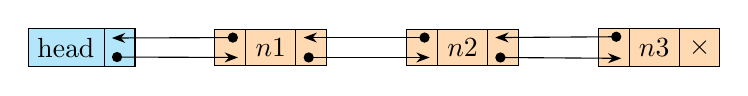
\begin{tikzpicture}[
    start chain,
    >=Stealth,
    ]

    \node[head node] (head) {head};
    \foreach \x in {n1,n2}{
      \node[list node] (\x) {\nodepart{two}$\x$};
    }

    \node[list node]
      (n3) {\nodepart{two}$n3$\nodepart{three}$\times$};

    \foreach \x/\y in {head/n1,n1/n2,n2/n3}{
      \draw[Circle->] ($(\x.-10)+(-0.3,0)$) -- ($(\y.190)+(0.3,0)$);
      \draw[Circle->] ($(\y.170)+(0.3,0)$) -- ($(\x.10)+(-0.3,0)$);
    }

  \end{tikzpicture}
\end{figure}


\end{document}
